\allowdisplaybreaks
\section{ARQ: Independent Retransmissions}\label{sec:arq}
Consider an ARQ retransmission scheme with independent failure events. The arrivals occur randomly with a probability $f$, forming a FIFO queue. Failed transmissions are added back to the head of the queue after $\delta$ slots, as described in Section~\ref{sec:model}. We first compute the wait delay and service delay separately and then derive the total delay. 

\subsection{Queing Model}
The UE buffer is modelled as a discrete-time Markov chain where the states represent the queue length, including the packet currently being served. State observations are made at the slot boundary. As mentioned in the system model, a departure occurs with every transmission attempt (with a probability of $1$). This is immediately followed, in order, by a retransmission schedule for failed packets, the slot boundary and the new arrivals. The retransmission is scheduled for a slot $\delta+1$ after the corresponding transmission slot. 

It is straightforward to see that the state transitions from state $q$ to $q+1$ corresponds to an arrival at the immediate next slot, say $k$, and a transmission failure at slot $k-\delta-1$. 
The transmission failure at slot $k-\delta-1$ is given by $p\left(1-\pi_0(1-f)\right)$ where $\pi_0$ denotes the probability of an empty queue. Here we take care of the fact that either the queue needs to be non-empty or there should be a fresh arrival for a transmission to happen in the first place to get a failed transmission.
Thus we obtain the Markov chain shown in Fig.\ref{fig:markovChain_modified}, where $\hat{p} = p\left(1-\pi_0(1-f)\right)$ and $\hat{p}' = 1-\hat{p}$. 
The residual self-loop probabilities of $1-f\hat{p}$ for state~0 and $f\hat{p}' + f'\hat{p}$ for all other states are not shown in the figure.

\begin{figure*}[t]
\centering
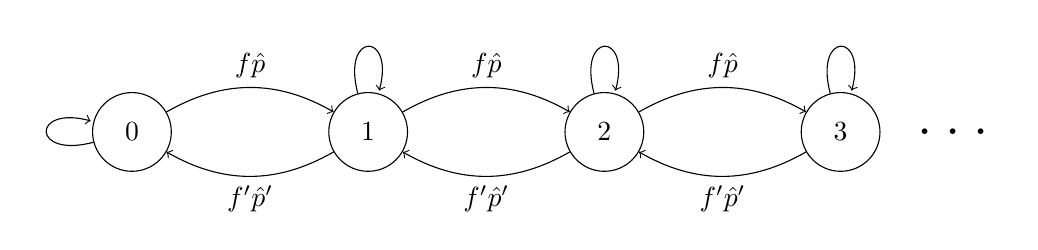
\begin{tikzpicture}
    % Define the nodes
    \node[draw, circle,minimum size=1cm] (s0) at (0,0) {0};
    \node[draw, circle,minimum size=1cm] (s1) at (3,0) {1};
    \node[draw, circle,minimum size=1cm] (s2) at (6,0) {2};
    \node[draw, circle,minimum size=1cm] (s3) at (9,0) {3};
    
    \node at (10.5,0) {\Huge\dots};
    % Arrows to the next state (curved up)
    
    \draw[->] (s0) to[bend left] node[midway, above] {$f\hat{p}$} (s1);
    \draw[->] (s1) to[bend left] node[midway, above] {$f\hat{p}$} (s2);
    \draw[->] (s2) to[bend left] node[midway, above] {$f\hat{p}$} (s3);

    % Arrows to the previous state (curved down)
    \draw[->] (s1) to[bend left] node[midway, below] {$f'\hat{p}'$} (s0);
    \draw[->] (s2) to[bend left] node[midway, below] {$f'\hat{p}'$} (s1);
    \draw[->] (s3) to[bend left] node[midway, below] {$f'\hat{p}'$} (s2);

    % Self-loop arrows
    \draw[->] (s0) edge[loop left] node[left] {} (s0);
    \draw[->] (s1) edge[loop above] node[above] {} (s1);
    \draw[->] (s2) edge[loop above] node[above] {} (s2);
    \draw[->] (s3) edge[loop above] node[right] {} (s3);
\end{tikzpicture}
\caption{Markov chain with queue length as states as observed at the slot boundary for an ARQ scheme. The transition probabilities, except the self-loop probabilities, are shown.}
\label{fig:markovChain_modified}
\end{figure*}


\subsubsection{Steady state probabilities}
We now focus on determining the steady-state probabilities (SSP) of the queue. Rather than directly finding the SSP of the initial Markov chain, we bound it using the SSP of a modified Markov chain representing an \textit{immediate feedback scenario} with $\delta = \ddecod = 0$, which is mathematically more tractable.

In such a scenario, the retransmission happens in the immediate next slot. One can alternatively consider that the departure occurs with a probability of $1-p$ instead of $1$, and there is no retransmission scheduled. 
The events between two state observations are an arrival at the start of the slot and a departure at the end of the slot with probabilities $f$ and $1-p$, respectively. 
Thus, the transition from state $q$ to $q+1$ comes with a probability $fp$, larger than $f\hat{p}$. 
Therefore, the CCDF of the queue length of this adapted Markov chain stochastically dominates that of the Markov chain from \ref{fig:markovChain_modified}. We will elaborate on this soon and use it to bind the violation probability of the wait delay. 

Let $\pi_i$ denote the steady-state probability of the adapted Markov chain. Lemma~\ref{lemma_arq_queue} provides the CCDS of the queue length.

\begin{lemma}\label{lemma_arq_queue}
    The CCDF of the queue length $Q$ is given by:
    \begin{equation}
        \mathbb{P}\left(Q>q\right) = \left(\dfrac{fp}{(1-f)(1-p)}\right)^{q+1}\label{eq:secARQ_QueueCCDF}
    \end{equation}
\end{lemma}
\begin{proof}
 \begin{align*}
    \pi_0 &= (1-fp)\pi_0 + f'p'\pi_1, \\
    \Rightarrow \pi_1 &= \dfrac{fp}{f'p'}\pi_0.\\
    \pi_1 &= fp\pi_0+ (1-fp-f'p')\pi_1+ f'p'\pi_2, \\
    \Rightarrow \pi_2 &= \dfrac{fp}{f'p'}\pi_1,\\
     &=  \left(\dfrac{fp}{f'p'}\right)^2\pi_0.
\end{align*}
Continuing with the same steps, we get
\begin{align*}
    \!\pi_i &= \left(\dfrac{fp}{f'p'}\right)^{i}\pi_0,\,\forall i\geq0,
    \intertext{that is,}
\!\pi_i &= \left(\dfrac{fp}{(1-f)(1-p)}\right)^{i}\!\!\left(1-\dfrac{fp}{(1-f)(1-p)}\right)\!,\forall i\geq0.\numberthis\label{eq:secARQ_ssp}
\end{align*}
Let $Q$ be the random variable denoting the queue length in the immediate feedback scenario, the distribution of which is given in \eqref{eq:secARQ_ssp}. Thus,
\begin{align*}
    \mathbb{P}\left(Q>q\right)&=\left(1-\dfrac{fp}{(1-f)(1-p)}\right)\\
    &\qquad\qquad\quad\sum_{i=q+1}^{\infty}\left(\dfrac{fp}{(1-f)(1-p)}\right)^{i},\,\forall i\geq0.\\
    &=\left(\dfrac{fp}{(1-f)(1-p)}\right)^{q+1}.
\end{align*}   
\end{proof}


% \paragraph*{Stability}
Observe that the queue is stable if the arrival rate does not exceed the departure rate, i.e. if $f \leq 1 - p$ or equivalently if $\frac{p}{1-f} \leq 1$. This can also be derived by computing the expected queue length $\Bar{\pi}$:
\begin{align*}
    \Bar{\pi} &=\left(1-\dfrac{fp}{(1-f)(1-p)}\right)\sum_{i=0}^{\infty}i\left(\dfrac{fp}{(1-f)(1-p)}\right)^{i},\\
    &=\left(1-\dfrac{fp}{(1-f)(1-p)}\right)\frac{(1-f)(1-p)}{(1-f-p)^2}fp,\\
    &=\frac{fp}{1-f-p},
\end{align*}
which implies stability when:
\begin{equation}
    \frac{p}{1-f}\leq1.\numberthis\label{eq:secARQ_zerofdbk_stability}
\end{equation}


\subsection{Wait delay}
It is clear from \eqref{eq:secARQ_QueueCCDF} that the queue length distribution of the immediate feedback scenario with PER $p$ stochastically dominates the queue length distribution of a delayed feedback scenario with a PER $\hat{p} < p$ in a first-order stochastic dominance sense~\cite{whang2019econometric}.


Let $\dwait\vert Q$ be the wait delay, conditioned on the queue length. Thus, 
\begin{align*}
    \mathbb{P}(\dwait =k)&=\sum_q\,\pi_q\mathbb{P}(\dwait ={k}\vert Q=q).
\end{align*}
As the wait delay increases with queue size, the stochastic dominance of the queue length of the delayed feedback scenario also implies the stochastic dominance of the corresponding wait delay. This will also become evident from Lemma~\ref{lemma_arq_wait}, where the upper bound, which is the CCDF of the wait delay with immediate feedback, decreases as the PER decreases. 
This upper bound is found to be sufficiently tight from simulations. This is because, unlike the service delay, the wait delay measured from arrival to the first transmission is largely unaffected by the feedback.


Recall that the sum of i.i.d. geometric random variables follows a negative binomial distribution\cite{johnson2005univariate}. 
For $X_{q}$ representing such a sum, the probability mass function is given by:
\begin{equation}
    \mathbb{P}(X_{q}=k)=\dfrac{(k-1)!}{(q-1)!(k-q)!}(1-p)^qp^{k-q}.\label{eq:secARQ_geoSum}
\end{equation}
% We now bound $\dwait$ by marginalizing the conditional distribution over steady-state queue probabilities.
 % \todo[inline]{Discuss more or prove mathematically the stochastic dominance?}
\begin{lemma}\label{lemma_arq_wait}
    The CCDF of the wait delay is given by:
    \begin{equation}
  \mathbb{P}(\dwait >k) \leq\frac{f}{1-p}\left(\frac{p}{1-f}\right)^{k+1}.\label{eq:secARQ_waitdelay} 
    \end{equation}
\end{lemma}
\begin{proof}
For the immediate feedback scenario, the number of transmissions attempted by a packet in the queue is distributed geometrically. Thus, $\mathbb{P}(D_w\vert Q)$ is given by the sum of $Q$ iid geometrically distributed random variables. We have,
\begin{align*}
\mathbb{P}(\dwait\!>\!j)&\leq 1\!-\!\left(\pi_0+\sum_{k=1}^{j}\sum_{q=1}^{k}\pi_q\,\mathbb{P}(D_w=k\vert Q=q)\right),\,\forall j\geq0.
\end{align*}
 Here, $\pi_0$ represents an empty queue. Let $Z(k)$ denote the inner sum. Expanding with \eqref{eq:secARQ_geoSum}, we have:
 \begin{equation}
Z(k)=\sum_{q=1}^{k}\pi_q\dfrac{(k-1)!}{(q-1)!(k-q)!}(1-p)^qp^{k-q},\,\forall k\geq1.
 \end{equation}
\begin{align*}
&=\sum_{q=1}^{k} 
\left( \frac{f \, p}{(1 - f) \, (1 - p)} \right)^q 
\left(1 - \frac{f \, p}{(1 - f) \, (1 - p)} \right)\\&\hspace{8em}
\left( \frac{(k - 1)!}{(k - q)!\,(q - 1)!} \right)
(1 - p)^q \, p^{k - q},\\
&=\left(1 - \frac{f \, p}{(1 - f) \, (1 - p)} \right)\sum_{q=0}^{k-1} 
\left( \frac{f \, p}{(1 - f) \, (1 - p)} \right)^{q+1} \\&\hspace{6em}
\left( \frac{(k - 1)!}{(k - q-1)!\,(q)!} \right)
(1 - p)^{q+1} \, p^{k - q-1},\\
% &=\left(1 - \frac{f \, p}{(1 - f) \, (1 - p)} \right)\sum_{q=0}^{k-1} 
% p^{q+1}\left( \frac{f}{(1 - f)} \right)^{q+1} 
% \left( \frac{(k - 1)!}{(k - q-1)!\,(q)!} \right) p^{k - q-1}\\
&=\left(1 - \frac{f \, p}{(1 - f) \, (1 - p)} \right)
p^{k}
\sum_{q=0}^{k-1} 
\left( \frac{f}{1 - f} \right)^{q+1}\\&\hspace{13em}
\left( \frac{(k - 1)!}{(k - 1 -q)!\,(q)!} \right),\\
&=\left(1 - \frac{f \, p}{(1 - f) \, (1 - p)} \right)
p^{k}\left( \frac{f}{1 - f} \right)
% \\&\hspace{12.5em}
\sum_{q=0}^{k-1} {\binom{k-1}{q}}
\left( \frac{f}{1 - f} \right)^{q},\\
&=\left(1 - \frac{f \, p}{(1 - f) \, (1 - p)} \right)
p^{k}\left( \frac{f}{1 - f} \right)
% \\&\hspace{15.5em}
\left(1+ \frac{f}{1 - f} \right)^{k-1},\\
% &=f\,\left( \frac{p}{1 - f} \right)^{k}
% \left(1 - \frac{f \, p}{(1 - f) \, (1 - p)} \right)\\
% \Rightarrow\mathbb{P}(\dwait >k) &= 1-\left(\pi_0+\sum_{i=1}^{k}\mathbb{P}(\dwait =k)\right)
&=f\,\left( \frac{p}{1 - f} \right)^{k}
\frac{1-f-p}{(1 - f) \, (1 - p)}.
\end{align*}
\begin{equation*}
 \Rightarrow\mathbb{P}(\dwait >j) \leq 1-\left(\pi_0+\sum_{k=1}^{j}Z(k)\right),  
\end{equation*}
\begin{align*}
% \Rightarrow\mathbb{P}(\dwait >j) &\leq 1-\left(\pi_0+\sum_{k=1}^{j}Z(k)\right)\\
&=1-\left(\pi_0+\sum_{k=1}^{j}f\,\left( \frac{p}{1 - f} \right)^{k}
\frac{1-f-p}{(1 - f) \, (1 - p)}\right),\\
% \Rightarrow\mathbb{P}(\dwait >j) &= 1-\left(\frac{1-f-p}{(1 - f) \, (1 - p)}+\sum_{k=1}^{j}f\,\left( \frac{p}{1 - f} \right)^{k}
% \frac{1-f-p}{(1 - f) \, (1 - p)}\right)\\
% \Rightarrow\mathbb{P}(\dwait >j) &= 1-\left(\frac{1-f-p}{(1 - f) \, (1 - p)}\right)\left(1+\sum_{k=1}^{j}f\,\left( \frac{p}{1 - f} \right)^{k}\right)\\
 &= 1-\left(\frac{1-f-p}{(1 - f) \, (1 - p)}\right)\left(1 + f\sum_{k=1}^{j}\left( \frac{p}{1 - f} \right)^{k}\right),\\
 &= 1-\left(\frac{1-f-p}{(1 - f) \, (1 - p)}\right)\\&\hspace{6em}\left(1 + \frac{fp}{1-f-p}\left(1-\left(\frac{p}{1-f}\right)^j\right)\right),\\
&= 1-\left(1-f-p+fp-fp\left(\frac{p}{1-f}\right)^j\right)\\&\hspace{13.5em}\left(\frac{1}{(1 - f) \, (1 - p)}\right),\\
&=\frac{fp}{(1-f)\,(1-p)}\left(\frac{p}{1-f}\right)^j,\\
&=\frac{f}{1-p}\left(\frac{p}{1-f}\right)^{j+1}.
\end{align*}
\begin{equation}
    \Rightarrow\mathbb{P}(\dwait >k) \leq\frac{f}{1-p}\left(\frac{p}{1-f}\right)^{k+1}.\nonumber
\end{equation}
\end{proof}

\subsection{Delay Violation Probability}\label{NoIR_dvp}
To get the DVP, we combine the upper bound of $\dwait$ with the service delay. The service delay is geometrically distributed based on the failure probability at the corresponding attempt, with values depending on $\delta$. It is given by:
\begin{align}
    \mathbb{P}\left(\dserv =k(\ddecod+1)+\delta(k-1)\right) &= p^{k-1}(1-p).\label{eq:secARQ_servDelay}\\
    \mathbb{P}\left(\dserv >k(\ddecod+1)+\delta(k-1)\right) &= p^{k}.\nonumber
\end{align}
Recall $k_d$ defined as the maximum number of transmissions possible before the service delay alone exceeds the delay target:
\begin{align}
    k_d\,\coloneqq& \underset{i}{Max}\,\left\{\,i:i(\ddecod+1)+(i-1)\delta\leq\left\lfloor\frac{d}{T}\right\rfloor\,\right\}\nonumber\\
    =&\left\lfloor\frac{\frac{d}{T}+\delta}{\delta+\ddecod+1}\right\rfloor.\label{eq:secARQ_kd}
\end{align}
\begin{theorem}\label{theorem_arq_dvp}
The DVP of the ARQ scenario for a delay target $d$ is given by:
\begin{multline}
\mathbb{P}(\dtot >d)\leq p^{ k_d } \\-  
\dfrac{f\,\left(\frac{p}{1-f}\right)^{  \left\lfloor\nicefrac{d}{T}\right\rfloor +\delta}
\left(1-p^{ k_d }\left(\frac{p}{1-f}\right)^{- k_d (1+\delta+\ddecod)}
\right)}
{1-f-\left(\frac{p}{1-f}\right)^{\delta+\ddecod}}.\numberthis\label{dvpbound}
\end{multline}
\end{theorem}
\begin{proof}
We have,
\begin{align*}
\mathbb{P}(\dtot >d)&\leq \sum_{i}\mathbb{P}(\dserv =i)\mathbb{P}(\dwait >d-i),\\
% &= p^{k_d} + \sum_{i=1}^{{ k_d }} (1 - p) p^{i - 1} \left( \sum_{k = 1 + \left\lfloor\nicefrac{d}{T}\right\rfloor - (i + (i - 1) {\delta})}^{\infty}f\,\left( \frac{p}{1 - f} \right)^{k}
% \frac{\left(1-f-p\right)}{(1 - f) \, (1 - p)}\right)
&= p^{k_d} + \sum_{i=1}^{{ k_d }} (1 - p) p^{i - 1}
\\&\hspace{2.5em}\left( \frac{f}{1-p}\left(\frac{p}{1-f}\right)^{1 + \left\lfloor\nicefrac{d}{T}\right\rfloor - \big(i(\ddecod+1) + (i - 1) {\delta}\big)}\right).
\end{align*}
The first term corresponds to the probability that the service delay alone exceeds the target. The second term accounts for a successful transmission at the $i^{\mathrm{th}}$ attempt with a service delay of $i(\ddecod+1) + (i-1)\delta$, along with all possible wait delays from \eqref{eq:secARQ_waitdelay} that in combination violate the delay target.
\begin{multline}
    \Rightarrow\mathbb{P}(\dtot >d) \leq p^{k_d} + 
f\left(\frac{p}{1-f}\right)^{1 + \left\lfloor\nicefrac{d}{T}\right\rfloor + \delta}\,
\\\sum_{i=1}^{{ k_d }}p^{i - 1} \left(\frac{p}{1-f}\right)^{-i(1+\delta+\ddecod)}
\end{multline}
\begin{align*}
&= p^{k_d} + 
f\left(\frac{p}{1-f}\right)^{1 + \left\lfloor\nicefrac{d}{T}\right\rfloor + \delta}\,
\\&\hspace{10.5em}\sum_{i=0}^{{ k_d -1 }} p^{i} \left(\frac{p}{1-f}\right)^{-(i+1)(1+\delta+\ddecod)}\\
&= p^{k_d} + 
f\left(\frac{p}{1-f}\right)^{1 + \left\lfloor\nicefrac{d}{T}\right\rfloor + \delta}\,
\left(\frac{p}{1-f}\right)^{-(1+\delta+\ddecod)}\,
\\&\hspace{10.5em}\sum_{i=0}^{{ k_d -1 }} p^{i} \left(\frac{p}{1-f}\right)^{-i(1+\delta+\ddecod)}\\
&= p^{k_d} + 
f\left(\frac{p}{1-f}\right)^{ \left\lfloor\nicefrac{d}{T}\right\rfloor-\ddecod}\,
\sum_{i=0}^{{ k_d -1 }} p^{i} \left(\frac{p}{1-f}\right)^{-i(1+\delta+\ddecod)}\\
% &= p^{k_d} + 
% f\left(\frac{p}{1-f}\right)^{ \left\lfloor\nicefrac{d}{T}\right\rfloor}\,
% \frac{1-\left(p\left(\frac{p}{1-f}\right)^{-(1+\delta)}\right)^{k_d}}{1-\left(p\left(\frac{p}{1-f}\right)^{-(1+\delta)}\right)}\\
&= p^{k_d} + 
f\left(\frac{p}{1-f}\right)^{ \left\lfloor\nicefrac{d}{T}\right\rfloor-\ddecod}\,
\frac{1-p^{k_d}\left(\frac{p}{1-f}\right)^{-k_d(1+\delta+\ddecod)}}{1-p\left(\frac{p}{1-f}\right)^{-(1+\delta+\ddecod)}}
% &= p^{ k_d } +  
% \dfrac{f\,\left(\frac{p}{1-f}\right)^{  \left\lfloor\nicefrac{d}{T}\right\rfloor +\delta}
% \left(1-p^{ k_d }\left(\frac{p}{1-f}\right)^{- k_d (1+\delta)}
% \right)}
% {\left(\frac{p}{1-f}\right)^{\delta}\left(1-p\left(\frac{p}{1-f}\right)^{-(1+\delta)}\right)}\\
\end{align*}
\begin{multline}
    \Rightarrow\mathbb{P}(\dtot >d)\leq p^{ k_d } \\-  
\dfrac{f\,\left(\frac{p}{1-f}\right)^{  \left\lfloor\nicefrac{d}{T}\right\rfloor +\delta}
\left(1-p^{ k_d }\left(\frac{p}{1-f}\right)^{- k_d (1+\delta+\ddecod)}
\right)}
{1-f-\left(\frac{p}{1-f}\right)^{\delta+\ddecod}}
\end{multline}
\end{proof}
% \todo[inline]{Outro?}







